مقدمه‌چینی، توجیه، توضیح و تعریف کافی است. وقت آن است که به خوراک اصلی
این کتاب برسیم - روندد واقعی تولید و تست یک پیش‌نمونه.

در ابتدا، انواع اولیه پیش‌نمونه سازی را برای شما معرفی می‌کنم و سپس به
راه‌های تست آنها نگاهی انداخته و در نهایت تمام آنچه را آموخته‌ایم را در
چند مثال کامل تجمیع می‌کنم.

\section{تکنیک‌های درهم برهم پیش‌نمونه
سازی}\label{ux62aux6a9ux646ux6ccux6a9ux647ux627ux6cc-ux62fux631ux647ux645-ux628ux631ux647ux645-ux67eux6ccux634ux646ux645ux648ux646ux647-ux633ux627ux632ux6cc}

روزی اگر این کتاب مبدل به یک \textbf{چیز} \emph{درست} شد، من سرمایه
زمانی بیشتری برای تولید ساختار سلسله مراتبی روش‌های پیش‌نمونه سازی میکنم
که بصورت کامل با ساختار درست و بصورت رسمی این تکنیک‌ها را ارائه می‌دهد.
در آن زمان به هر روش یک نام فانتزی داده، سناریو ایده‌آل استفاده از آن را
ارائه کرده و مثال‌های بسیاری میزنم. اما از آنجایی که خود این کتاب هنوز
یک پیش‌نمونه است، چیزی شما خواهید دید یک لیست درهم برهم از روش‌ها به
همراه توصیف خام اینکه هر روش کی و چگونه مورد استفاده قرار می‌گیرد.

لیست خلاصه این روش‌ها که قرار است در مورد آنها صحبت کنیم از قرار زیر
است:

\begin{itemize}
\item
  \textbf{ترک مکانیکی} - انسان‌ها را جایگزین کامپیوترها یا ماشینهای
  پیچیده و گران قیمت کنید.
\item
  \textbf{پینوکیو} - نسخه غیر عملیاتی و «مرده» محصول خود را بسازید.
\item
  \textbf{استانی} - قبل از اینکه در کل جهان محصول خود را ارائه کنید،
  آنرا روی مجموعه کوچکی تست کنید.
\item
  \textbf{در جعلی} - یک «ورودی» جعلی برای محصولی که اصلا وجود خارجی
  ندارد بسازید.
\item
  \textbf{وانمود کنید که دارید} - قبل از سرمایه گذاری برای خرید هر چیزی
  که برای \textbf{چیز}تان به آن نیاز دارید، آنرا قرض گرفته یا اجاره
  کنید.
\item
  \textbf{لیبل گذاری مجدد} برچسب جدید روی محصول فعلی که شبیه آن چیزی است
  که شما میخواهید آنرا تولید کنید بگذارید.
\end{itemize}

در استفاده، سوء استفاده، استفاده غلط یا استفاده نابجا از هریک از این
تکنیک‌ها آزاد هستید.آنها را ترکیب، پالایش، باز تعریف نموده و آنها را به
دانش شخصی خود اضافه کنید. اگر شما یک روش جالب پیش‌نمونه سازی پیدا کرده و
یا پیشنهادی در این مورد دارید حتما من را در جریان قرار دهید. آنرا توصیف
نموده و به آن نامی بدهید و ممکن است من آنرا در نسخه بعدی کتاب بگنجانم یا
در وبلاگم آنرا ارائه دهم.

حالا نوبت توضیح بیشتر در مورد هر تکنیک است.

\section{ترک
میکانیکی}\label{ux62aux631ux6a9-ux645ux6ccux6a9ux627ux646ux6ccux6a9ux6cc}

این تکنیک پیش‌نمونه سازی نامش را از یک «ماشین» بازی شطرنج به همین نام
قرض گرفته است. این ماشین در انتهای قرن ۱۸ میلادی در سراسر دنیا به نمایش
گذاشته شد. به مردم قبولانده می‌شد که «ترک» یک ابداع مکانیکی است که
برنامه ریزی شده تا شطرنج بازی کند. در واقع، درون جعبه یک شطرنج باز با
استعداد و کوچک قرار داشت که با استفاده از دسته‌های ماشین شطرنج بازی
می‌کرد.

\begin{figure}[htbp]
\centering
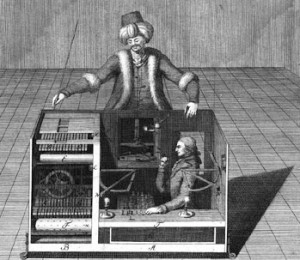
\includegraphics{mechanicaltork.png}
\caption{ترک میکانیکی}
\end{figure}

پیش‌نمونه‌های ترک میکانیکی برای موقعیت‌هایی که می‌توان انسان را بصورت
مخفی جایگزین تکنولوژی‌های پرهزینه، پیچیده یا نیازمند توسعه در آینده کرد
ایده‌آل است. آزمایش تبدیل متن به گفتار آی بی ام نمونه به نقصی از این روش
است. توسعه یک موتور تبدیل متن به گفتار سالهای زمان و سرمایه گذاریی عظیمی
نیاز داشت اما یک تایپیست انسانی که در اتاق کناری مخفی شده بود به راحتی
این کارایی پیچیده را شبیه سازی کرد. همانند شطرنج باز درون ترک میکانیکی.

\section{پینوکیو}\label{ux67eux6ccux646ux648ux6a9ux6ccux648}
